\section{Introduction}\label{sec:intro}
% Revision 2 by the lead and Claude, 2026-11-26. Addresses REVIEW_LOG round 1: the 12 intro items, M2-M6, M9-M10, minor 1 and 14,
% and fills the v8 TODO. Rules: numbers only through macros; each claim maps to a confirmed or decided locked prediction (CL ids in
% the comments); exploratory results appear only as caveats or pointers. Contribution 2 says "prove": the proofs of Propositions 1-3
% in Appendix C must be complete before the second review.
% Figure 1(a): change the label of the bottom row inside figs/fig1.pdf to "state write (RRR-16 / C3-U4)" (M10).

\begin{figure}[t]\centering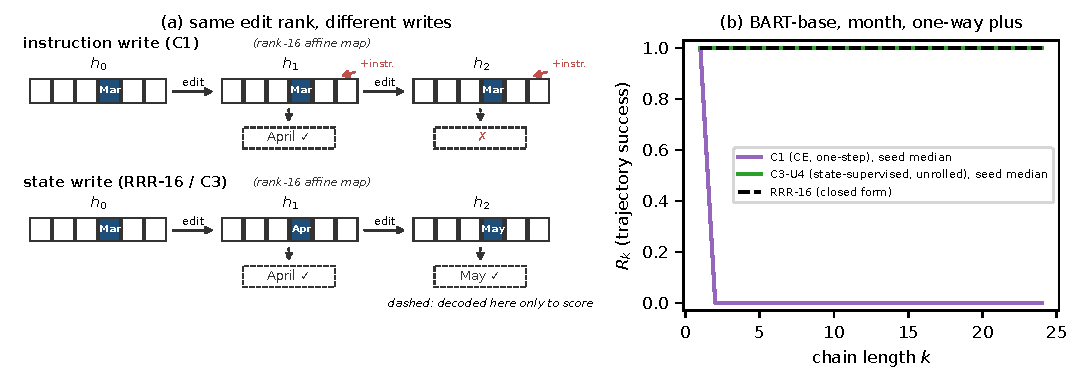
\includegraphics[width=\linewidth]{figs/fig1.pdf}
\caption{\textbf{Decodable is not composable.} (a) Two rank-16 affine edits of the same encoder states both decode correctly after
one step. The decoder-trained edit (top) writes an instruction and leaves the slot at the source state, so the second edit fails; the
state-writing edit (bottom; the closed-form RRR-16 or the unrolled, state-supervised C3-U4) moves the slot and composes. Intermediate
states are decoded here only to score the chain; a pipeline that passes latents on never decodes them. (b) BART-base, month, one-way
plus chains: C1 fails from the second step; RRR-16 and C3-U4 compose.}\label{fig:fig1}
\end{figure}

Methods that edit a model's internal representations, rather than its inputs or weights, are usually judged by a single round trip:
apply the edit once, decode, and check that the output changed as intended~\citep{turner2023actadd,zou2023repe,li2023iti}. A growing
number of systems, however, pass latent states on without decoding them: a server that computes on encrypted representations cannot
read the states it transforms~\citep{chen2022thex}, models exchange key--value caches instead of text~\citep{fu2026c2c}, and reasoning
can be carried out in a continuous latent space~\citep{hao2024coconut}. In such pipelines an edited state is edited again or handed to
another component, and no one inspects the states in between. What matters there is not whether one edit decodes correctly but
whether edits \emph{compose}: applying an edit $k$ times should move the underlying variable by $k$ steps.

We study when latent edits compose in a setting where composition can be measured exactly. Each input sentence to a frozen
encoder--decoder model contains a \emph{slot}, a word that takes one of $N$ cyclically ordered states such as a weekday or a month.
An edit maps the encoder states so that the decoder produces the same sentence with the state moved by one; a \emph{chain} applies the
edit repeatedly, and we decode after every step only to score it. Our main backbones are BART-base and T5Gemma 2B--2B on templated
sentences; we also test natural sentences and T5Gemma 9B--9B. Outside the binding experiments, every editor is a rank-limited affine
map of the encoder states, so differences between editors come from how they are fitted, not from what they can represent.

\paragraph{Decodable is not composable.}
\claim{CL1}\claim{CL2}\claim{CL3}\claim{CL4}\claim{CL17}\claim{CL18}%
An editor trained through the decoder to produce the target sentence after one step (C1) is correct on every BART-base confirmation
world after that step (step-1 success \CLoneVfiveCOneRoneMin), yet no chain survives the second step ($\Rk{2}=\CLoneVfiveCOneRtwoMax$);
the same happens on natural text with both backbones and at 9B--9B ($\Rk{2}=\CLseventeenCOneRtwoMax$ and \CLeighteenCOneRtwoMax). A
closed-form operator of the same form, fitted only to pairs of encoder states, composes: its one-way $\Rk{2N}$ is
\CLoneVfiveBaseMin{} in every single-template backbone--domain combination (rank 16, or 32 for hour on T5Gemma;
Figure~\ref{fig:fig1}). C1's objective asks only for the right output after one step, so its failure is permitted; the point is that
the usual one-step check cannot tell it apart from an operator that composes. The difference lies in what the edits write. C1 writes
an \emph{instruction} that the decoder executes once, rather than a state that a later edit can act on: its writes are highly similar
across source states (median cosine \CLtwoWriteCosSource), almost unaligned with the change between the canonical encodings (median
cosine \CLtwoWriteCosCanon), and a linear probe still reads the source state from the edited latent (\CLtwoProbeSource). Training
through longer chains does not remove this shortcut but replaces it with a step counter that fails just past the training horizon, even
when the horizon covers a full cycle. Adding a target for the state itself makes unrolled editors compose (one-way $\Rk{2N}$
\CLfourTfiveCThreeUfour{} on T5Gemma 2B--2B and \CLeighteenCThreeMin{} at 9B--9B; Section~\ref{sec:instructions}).
% CL1, CL2, CL3, CL4; CL17 (N3), CL18 (G1, G6)

\paragraph{What composable edits preserve.}
\claim{CL5}\claim{CL7}\claim{CL10}%
Decomposing the centred slot representations into harmonic planes, as found for cyclic features in language
models~\citep{engels2025notall,karkada2026symmetries}, turns composition into testable predictions. The slowest plane, the fundamental,
fixes the state's global position but changes least from one state to the next: its one-step energy was the smallest of all planes in
every backbone--domain combination we measured, and a locked test confirmed this at 9B--9B. On ideal codes a least-squares fit of limited
rank therefore drops the fundamental first (Proposition~2). Freezing the fundamental produces a signature we specified before the
confirmation runs: one-way chains fail as the displacement grows, alternating chains survive, and chains recover after $N$ steps. It
held in all \CLfiveVoneN{} locked single-template cells, on natural text and at 9B--9B; on held-out templates one alternating test
missed its threshold because the unfrozen operator itself is weaker there. Reserving rank for the fundamental repairs rank-deficient
operators on T5Gemma 2B--2B (one-way $\Rk{2N}$ from at most \CLtenRRRMax{} to \CLtenFFMin{} in all \CLtenCells{} cells), only partly
on BART-base, and not at 9B--9B (Section~\ref{sec:fourier}).
% CL5 (V1, V2a; N4; G3), CL7 (G4), CL10 (Q16); limitations: v6 M3, CL10 partial, 9B FF descriptive

\paragraph{Predicting composability without decoding the chains.}
\claim{CL8}\claim{CL9}%
Because composability is a property of the latent trajectory, it can be predicted without decoding the chains. We apply the edit to
encoder states only and, after every step, read the slot by comparing its harmonic coordinates with those of the clean encodings of
each candidate state; the plane weights of this readout are calibrated once on decoded development probes. On fresh worlds the readout
agrees with the decoded outcome of \CLeightAgreeBart{} (BART-base) and \CLeightAgreeTfive{} (T5Gemma) of chains, over all editors not
trained through the decoder, against \CLeightNaiveBart{} and \CLeightNaiveTfive{} for the naive rule that a chain succeeds whenever
its first step decodes. It reaches \CLseventeenAgreeBart{} and \CLseventeenAgreeTfive{} on natural text and \CLeighteenAgree{} at
9B--9B. Most of this gain is at the level of cells: an oracle that gives every chain the majority outcome of its cell already reaches
\CLeightMajBart{} and \CLeightMajTfive{}, and Section~\ref{sec:prediction} analyses where the readout errs. One decoded step suffices to
tell the two kinds of editor apart: the step-1 disagreement between the readout and the decoded state separates the decoder-trained from
the state-supervised editors in all \CLnineCE{} and \CLnineState{} cells, and in all \CLeighteenDsepCells{} cells at 9B--9B.
% CL8 (L1, L2; N5; G5), CL9 (L3a-c; G5); caveat: majority reference (exploratory)

\paragraph{Scope.}
\claim{CL13}\claim{CL14}\claim{CL17}\claim{CL18}%
Slot-centred operators fitted on one set of templates also compose on held-out templates (one-way $\Rk{2N}$ between
\CLfourteenBaseHour{} and \CLfourteenBaseMonth{}), although alternating chains, and on T5Gemma the readout, are less reliable there. On
\CLseventeenWorlds{} natural sentences that mention a month, the slot operator composes on both backbones, and the instruction writes,
the freeze signature and the readout all carry over. At 9B--9B every locked prediction holds except one: composition switches on less
sharply below the predicted rank than predicted for month (RRR-9 one-way $\Rk{2N}=\CLeighteenRnineMonth$).
Section~\ref{sec:scope} also reports an exploratory pilot on a decoder-only model. The findings do not extend to edits that must look
content up elsewhere in the sentence. For binding edits, which move a pointer to the next listed participant, the best editor we
trained survives 30 steps on \CLthirteenSurvivors{} of eight seeds but has decayed by 100 steps on all of them
($\Rk{100}\le\CLthirteenHundredMax$); an editor given oracle routing has decayed by 30 steps (median $\Rk{30}=\CLthirteenOrEightThirty$).
% CL13 (K5, K7), CL14 (M1), CL17 (N1, N3-N5), CL18 (G1-G6, G2 counter-example)

\paragraph{Contributions.}
\begin{itemize}
\item We show that one correct decoding step does not imply composability, and trace the gap to editors that write instructions for the
decoder instead of states (Sections~\ref{sec:phenomenon}--\ref{sec:instructions}).
\item We identify what composable low-rank edits preserve in these domains---the harmonic planes of the slot code, including the
fundamental that a rank-limited fit drops first---and prove the rank bound and the freeze signatures for ideal codes
(Section~\ref{sec:fourier}, Appendix~\ref{app:theory}).
\item We predict composability without decoding the chains, and give a one-step test that tells decoder-trained from state-supervised
editors apart (Section~\ref{sec:prediction}).
\item All confirmatory results come from \CLmetaRounds{} preregistered rounds, on templated and natural text and up to T5Gemma 9B--9B;
exploratory analyses are marked as such, and Appendix~\ref{app:protocol} lists every locked prediction, including those that failed.
\end{itemize}
